\documentclass[10pt]{beamer}
%%% Pour le français %%%
\usepackage[utf8]{inputenc}
\usepackage[T1]{fontenc}
\usepackage[frenchb]{babel}
%%%%%%%%%%%%%%%%%%%%%%%%
% \usepackage{fancyhdr} % En-tête et pied de page personnalisés
% \usepackage{listings} % Pour du beau code coloré
%%%% Pour des maths %%%%
\usepackage{mathtools} % Pour pleins de commandes avec des maths
\usepackage{amssymb} % Pour les symboles
\usepackage{amstext} % Pour utiliser \text
% \usepackage{mathrsfs} % 3 fonts pour les 26 lettres
% \usepackage{amsthm} % Custom des theoremes
% \usepackage{tikz} % Pour des graphiques
%%%%%%%%%%%%%%%%%%%%%%%%
% \usepackage{layout} % Pour afficher le gabarit de mise en page
% \usepackage{geometry} % Pour régler les marges
% \usepackage{setspace} % Pour modifier l'interligne
% \usepackage{ulem} % Pour souligner et barrer du texte
%%% Pour des polices %%%
% \usepackage{bookman}
% \usepackage{charter}
% \usepackage{newcent}
% \usepackage{lmodern}
% \usepackage{mathpazo}
% \usepackage{mathptmx}
%%%%%%%%%%%%%%%%%%%%%%%%
% \usepackage{url} % Pour citer des urls
% \usepackage{graphicx} % Pour travailler sur des images
% \usepackage{color} % Pour manipuler les couleurs et colorer le texte
\usepackage{enumitem}

\title[TIPE — Optimisation des transports]{TIPE \\ Optimisation des transports}
\author{ROCHER Kilian — WILLEM Logan}
\date{2020 - 2021}

\mode<presentation>

\useoutertheme[footline=authortitle]{miniframes}
\useinnertheme{circles}
\usecolortheme{whale}
\usecolortheme{orchid}

\definecolor{beamer@blendedblue}{rgb}{0.137,0.466,0.741}
\definecolor{titleColor}{RGB}{102,153,255}
\definecolor{textColor}{RGB}{60,60,60}

\setbeamercolor{titlelike}{bg=titleColor}
\setbeamercolor{titlelike}{parent=structure}
\setbeamercolor{frametitle}{fg=black}
\setbeamercolor{title}{fg=black}
\setbeamercolor{item}{fg=black}
\setbeamercolor{normal text}{fg=textColor}
\setbeamertemplate{background canvas}[vertical shading][top=cyan!7!white,bottom=cyan!2!white]
\setbeamertemplate{blocks}[rounded][shadow=true]
\setbeamercolor{prop_low}{bg=red!10,fg=black!90}
\setbeamercolor{prop_up}{fg=white,bg=red!90}
\setbeamercolor{data_low}{bg=gray!10,fg=black!90}
\setbeamercolor{data_up}{fg=white,bg=gray!90}


\begin{document}
	\begin{frame}[plain]
		\maketitle
	\end{frame}

	\begin{frame}[plain]
		\tableofcontents
	\end{frame}

	\section{Situation du problème}
	
	\subsection{Qu'est ce que l'optimisation des transports?}
	
	\begin{frame}
		Définition et enjeux de l'optimisation des transports
	\end{frame}
	
	\subsection{Quelques exemples}
	
	\begin{frame}
		Quelques exemples de transport optimal avec images explicatives
	\end{frame}
	
	\section{Problème de tournée des véhicules}
	
	\subsection{Contexte}
	
	\begin{frame}
		Dans ce type de problèmes, il s'agit de minimiser le coût total (en distance par exemple) de la tournée de tous les véhicules, ayant pour objectif de livrer un nombre défini de clients.
	\end{frame}

	\subsection{Variantes}
	
	\begin{frame}
		\underline{Différentes variantes du problème de tournée des véhicules}
		\begin{itemize}[label=—]
			\item Classique (VRP) \pause
			\item Contrainte de capacité (CVRP) \pause
			\item Dépôts multiples (MDVRP) \pause
			\item Retours des colis (VRPPD et VRPB) \pause
			\item \dots \pause
		\end{itemize}
		\ \newline On s'est intéressé à la variante classique afin de s'approprier au mieux le problème.
	\end{frame}
	
	\section{Première résolution}

	\subsection{L'algorithme de Clarke \& Wright}

	\begin{frame}
		\begin{beamerboxesrounded}[upper=data_up,lower=data_low,shadow=true]{Données} \pause
			\begin{itemize}[label=-]
				\item $D$ : Dépot de coordonnées $(0,0)$\pause
				\item Une famille de points \((i_1,...,i_k) \in {(\lbrack-100,100\rbrack^2)}^k\) pour un certain $k \in \lbrack2,+\infty\lbrack$ représentant les clients\pause
				\item Une fonction $d$ qui calcule la distance entre deux points. \pause
			\end{itemize}
		\end{beamerboxesrounded}\ \newline
		\underline{Remarque} : Dans cette méthode de résolution, le nombre de véhicules n'est pas fixé. C'est l'algorithme qui décide du nombre optimal de véhicules à utiliser. 
	\end{frame}
	 
	\begin{frame}	
		\begin{definition}[Fonction \textit{gain}]
			On introduit la fonction $s$ qui calcule le gain après raccord de deux routes. Celle-ci calcule, pour deux points $i$ et $j$, la différence entre le chemin $D-i-D$ + $D-j-D$ qui vaut donc $2d(D,i) + 2d(j,D)$ au chemin $D-i-j-D$ donc la distance vaut $d(D,i) + d(i,j) + d(j,D)$
		\begin{align*}
			s(i,j) &= 2d(D,i) + 2d(j,D) - \lbrack d(D,i) + d(i,j) + d(j,D)\rbrack \\
			s(i,j) &= d(D,i) + d(j,D) - d(i,j)
		\end{align*}		
		\end{definition}
	\end{frame}

   \begin{frame}
       \begin{itemize}[label=-]
          \item Étape 1:
          \item Étape 2:
	   \end{itemize}
	\end{frame}

	\begin{frame}
		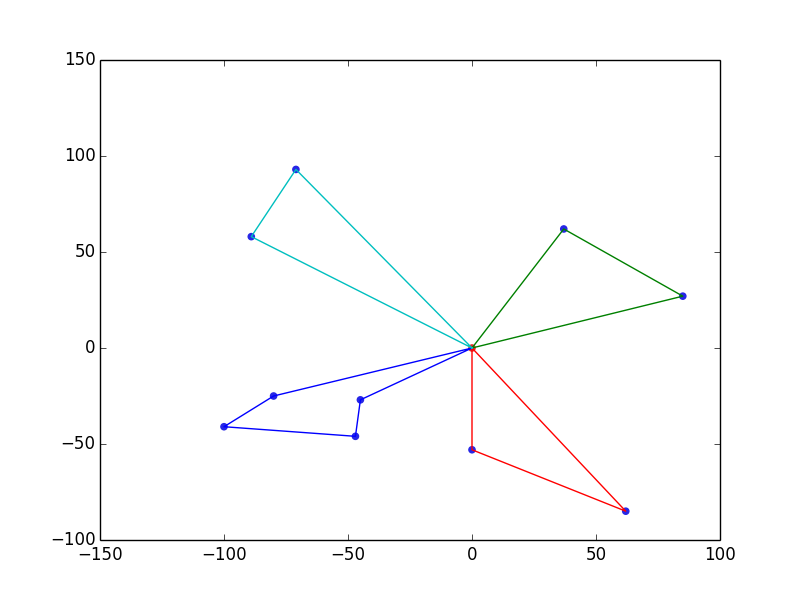
\includegraphics[scale=0.5]{Resultats/Cas Parfait.png}
	\end{frame}

	\subsection{Insuffisance de l'algorithme}
	   
	\begin{frame}
		Images de cas de croisements (même avec peu de clients)
	\end{frame}

	\section{Amélioration}

	\subsection{Le 2-opt}

	\begin{frame}
		Principe du 2-opt et résultats combinés
	\end{frame}

	\subsection{Comparaison des algorithmes}

	\begin{frame} 
		Différents résultats, comparaison et mise en avant du problème soulevé par le 2-opt (cas des trois points)
	\end{frame}

\end{document}